\externaldocument{tech_eclipse_text}

\section{Set-up and Terminology \label{terminology}}
The eclipse mapping program described in this paper derives a model for the relative surface brightness of a transiting planet host star when given a single band, short cadence light curve of the target as an input. Each iteration of the program produces a static map of the stellar surface. By applying the code to a series of short segments of the light curve, we are able to extract information about the time evolution of the star's surface brightness \cite{Huber2009}.  

In order for the program to create a brightness map, certain physical properties of the star and the planet must be provided. Stellar rotation period ($P_{rot}$), limb-darkening coefficients, orbital period ($P_{orb}$), orbital separation ($a$), impact parameter ($b$), and transit duration are all required in order for the program to produce an adequate model of the physical system. The star is assumed to be a rotating, uniform, solid body. In addition, the spin-axis of the star is required to be aligned with the orbital axis of the planet. The planet must also be on an approximately circular orbit. These criteria are both met for our test object, Kepler-17 \cite{Borucki2011}.

%Possibly move this next paragraph or restructure it. 
Other inputs to the code include the binning cadence for both in and out-of-transit points of the light curve, the number of boxes ($n_b$) and stripes ($n_s$) there should be in the surface map, number of days per individual brightness solution or {\it window}, and the number of days to increment each window.

The data is binned according to two separate binning cadences. In-transit points give information about smaller scale features, so they are binned at a high cadence. The out-of-transit points are binned at a low cadence because the overall longterm variability of a longitude can be tracked well with less information. Added benefits of binning the out-of-transit points at a low cadence are that the run-time of the code decreases with fewer points to match in the light curve and there is some degree of inherent noise removal by binning. Care must be taken at the boundaries of in- and out-of-transit regions of the light curve. Some bins will be cut off with fewer points in order to properly switch between the two different binning cadences.

In order to efficiently describe the details of our program, the geometry of the problem must be defined and some basic terminology must be established. The stellar surface is divided into a series of large {\it regions}, as shown in Figure~\ref{CoRoT}. While describing our program in this paper, the regions along the line of transit will be called {\it boxes}; the total longitudinal regions will be called {\it longitudes}; and the longitudinal regions with the box areas subtracted will be referred to as {\it stripes}. When talked about as an ensemble or when the distinction is unimportant, these regions will be referred to as just that - {\it regions}.

\begin{figure}[h]
	\centering
	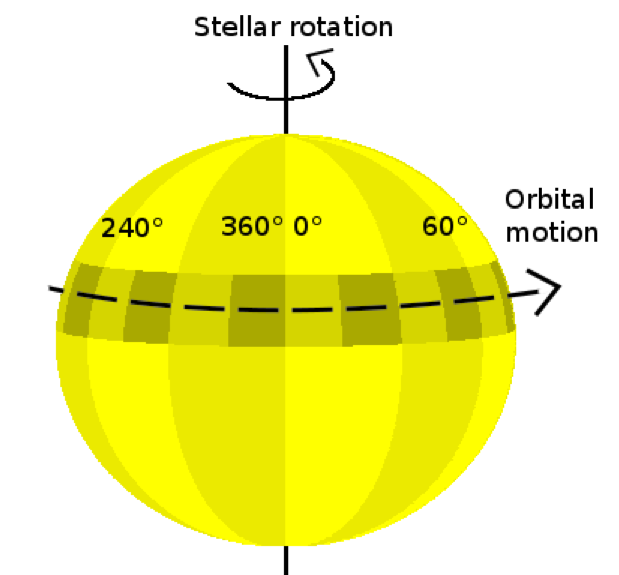
\includegraphics[width=.5\textwidth]{images/modelGeometry.png}
	\caption{A typical setup for a brightness map produced by the code. \cite{Huber2009}}
	\label{CoRoT}
\end{figure}

Our program calculates the model flux at each time step, by summing over the surface of the visible sphere according to:

\begin{equation}
	\fmod = \sum_j V_{i,j}b_j, 
\end{equation}

where $b_j$ is the brightness per unit area for region $j$ and $V_{i,j}$ is the {\it visibility} of region $j$ at time, $i$. Visibility is a measure of projected surface area along the line of sight. Eclipses are included in the visibility. When the planet occludes part of the star, the relative visible area of the star decreases. The eclipse is accounted for by subtracting the area that the planet obscures of a given box from the normal visibility of the same box at the given time step. Done this way, the transit produced in the model light curve is a box-car transit shape. To give a more smooth and realistic transit curve, limb-darkening is included according to the quadratic limb darkening law provided in \cite{Claret2004}.

The Amoeba Algorithm is a minimization tool that works well for small numbers of dimensions (regions in this case) and which will always converge to some minima (although not necessarily absolute) \cite{NR}. It determines the brightness values given pre-defined visibilities as described in section~\ref{vis}. Both of these, brightness values and visibilities, apply to a set of $j = n_{boxes} + n{stripes}$ regions. The planet will occlude only the boxes and will do so only during a transit. The longitudes' brightness values are defined as:

\begin{equation}
%Z_j = \frac{S_j - \frac{c}{q} \sum_{j=1}^{q}B_j}{1- c}
S_j = Z_j (1 - c) + \frac{c}{q} \sum_{j=1}^{q}B_j
\label{z_val}
\end{equation}
%Changed the above equation... switched Z and S values. So make sure that you switch the explanation in the next paragraph

%Summarize more generally what happens in the model flux...
%Explain visibilities, transit models, model flux, chi squared, amoeba. "I'm describing in more detail how each of these works in the following subsections."

Where $q$ is the ratio of $n_{boxes}$ to $n_{stripes}$ and $c$ is the ratio of the total eclipsed area to the non-eclipsed area. $c$ can be calculated by the same set of integrals that will be used for the visibilities. The Amoeba algorithm is given the set of box and longitude visibilites $\{b_1, ..., b_j, z_1, ..., z_n\}$. When the planet is not transiting, the only information available is about the total longitudinal brightness information. Within the chi-squared call of the Amoeba algorithm, the box and stripe visibilities and brightnesses are calculated as a way to blend the parameters together and get information about the overall longitude. This allows the use of boxes and stripes whose sum can be thought of as the longitude values in the Amoeba while still getting information about the boxes and the longitudes independently. This is called parameter interdependence. This appears to encourage the Amoeba Algorithm to navigate to a better local minima than if this process of creating parameter interdependence and using optimal variables were omitted. 



%The longitude values from equation~\ref{z_val} create parameter independence by changing the way that our algorithm navigates the chi-squared space so that such a case is less likely to become a local minimum. The Amoeba algorithm takes the set of box brightness guesses and longitude brightness guesses as inputs. During each call of the chi-squared algorithm the stripe values are calculated from the longitudes and boxes. The boxes and the stripes are then used to calculate the model flux.


















